\section{Propuesta}
Para garantizarle al usuario que la aplicación que implementa respeta
determinadas políticas de seguridad, el desarrollador Android requiere de una
herramienta que le permita: primero definir las políticas de seguridad a
evaluar, y segundo, verificar el cumplimiento de las políticas
definidas.\newline 
Así pues, la propuesta para cumplir con tales requerimientos consiste en proveer
una herramienta de análisis de flujo de información, mediante en el sistema de
anotaciones del lenguaje tipado de seguridad Jif. Se propone partir de Jif
porque este ofrece un sistema de anotaciones basado en un modelo de
etiquetas(DLM), más un módulo de verificación(compilador de Jif),
tal como se ilustra en la figura \ref{fig:desingReal}.
De este modo, con anotaciones en el código de su aplicación, el desarrollador
puede definir políticas de seguridad, para luego validar con el módulo de
verificación, si la aplicación respeta tales políticas.\newline 
Ahora bien, el principal reto para llevar a cabo dicha propuesta, es permitir el
análisis de flujo de información de aplicativos Android con el sistema de
anotaciones de Jif, puesto que, Jif sólo permite el análisis de flujo de
información en aplicativos Java convencionales, y una de las diferencias entre
una aplicación Android y una aplicación Java convencional es la API de Android,
puesto que, para adquirir sus funcionalidades una aplicación Android requiere de
clases de la API. No obstante, el sistema de anotaciones de Jif está
implementado para clases del lenguaje Java estandar y no para clases de la API
Android.\newline 
En consecuencia, el diseño ideal para contribuir con la solución del problema es:
una herramienta que contenga el setup de Jif para Android, e integre un clasificador de sources
y sinks. De modo que, la herramienta analice flujos de información en
aplicativos Android, verificando que cumplan con las políticas de seguridad que
el desarrollador ha definido.\newline 
El Setup de Jif para Android hace referencia a las clases de la API Android con
anotaciones Jif(Anotaciones a la API), estas anotaciones son necesarias porque
es a través de la API que la aplicación escribe o lee información de los sources
y los sinks, generando flujos de información entre los mismos. Por ende, el
análisis de flujo de información entre sources y sinks con el sistema de
anotaciones de Jif, implica anotaciones a clases de la API. 

Si bien, el diseño ideal requiere anotaciones a toda la API, para efectos del
presente trabajo se limita el Setup de Jif, partiendo de una política de
seguridad específica.
Por consiguiente, el diseño se centra en soportar un conjunto reducido de clases
de la API de Android, y en incluir un conjunto específico de sources y
sinks; de acuerdo a una política de seguridad establecida. Ese conjunto de
sources y sinks, se toma del listado de sources y sinks proveído por SuSi
\ref{sec:susi}.\newline
Adicionalmente, para aspectos de evaluación, se incluye el diseño de un anotador
que automatiza la anotación requerida por el desarrollador.
De modo que, acorde a la política de seguridad establecida, se genere la
versión anotada del aplicativo a analizar.\newline
La figura \ref{fig:desingReal} muestra el esquema del diseño, allí los componentes
principales son el \emph{generador de anotaciones} y la \emph{herramienta de
análisis estático}.\newline 
Para retornar la versión Jif del aplicativo, el \emph{generador de anotaciones}
parte del código fuente de la aplicación Android a analizar, la política de
seguridad a evaluar, y los sources y sinks requeridos para verificar tal
política.\newline 
Luego esa versión Jif del aplicativo se debe pasar como entrada a la herramienta
de análisis estático, la cual retorna el análisis de flujo de
información.\newline 
La \emph{herramienta de análisis estático}, está integrada
por el compilador de Jif(Módulo de verificación) y las anotaciones a la API de
Android.

\begin{figure}[t!]
	\begin{center} 
	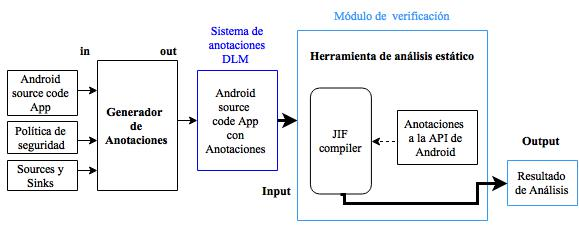
\includegraphics[width=8.8cm]{desing3Real-2-2-colors-2.jpg} 
	\end{center}
	\caption{Diseño herramienta de análisis estático.\newline
	Partiendo del código fuente del aplicativo Android, la política de seguridad a
	evaluar, más los sources y sinks requeridos para verificar la política; el
	generador de anotaciones retorna la versión anotada del aplicativo a analizar.
	Luego la versión anotada del aplicativo se pasa como entrada a la herramienta
	de análisis estático, la cual retorna el resultado de análisis de flujo de información.}
	\label{fig:desingReal}
\end{figure}

Siguiendo el esquema de diseño anteriormente descrito: primero, se define la
política de seguridad a evaluar \ref{subsection:politica}; segundo, se toman a
consideración elementos influyentes para verificar el cumplimiento de la
política mediante Jif \ref{subsec:consVerPol}; y tercero, teniendo en cuenta
\ref{subsection:politica} y \ref{subsec:consVerPol}, se definen los lineamientos
de anotación \ref{sec:lineamientos}. Tales lineamientos establecen el esquema
para anotaciones a la API Android y anotaciones a los aplicativos a
analizar(lineamientos del anotador).

\subsection{Definición de la política de seguridad}
% \textit{Definición de la política de seguridad}:
Detectar si una aplicación Android presenta flujos de información entre:
información con nivel de seguridad alto e información con nivel de seguridad bajo.\newline
\textit{Información con nivel de seguridad alto}: la información
catalogada con nivel de seguridad alto hace referencia a un conjunto de sources.
Los sources representan información confidencial o privada del usuario, por
tanto, el usuario quisiera tener el control de hacia donde se dirige tal
información.
El conjunto de sources está integrado por los métodos getDeviceId,
getSimSerialNumber, findViewById, getLatitude, getLongitude y getSubscriberId.
Adicional a estos métodos, se incluye el tipo de dato EditText, si y sólo si, el
campo UI al que hace referencia corresponde a un campo tipo textPassword(campos
destinados a almacenar contraseñas).\newline 
\textit{Información con nivel de seguridad bajo}: la
información considerada con nivel de seguridad bajo, comprende un conjunto
de sinks. Los sinks son canales que permiten la salida de información del
dispositivo, por ejemplo, los mensajes de texto. El conjunto de sinks
está integrado por los métodos de la clases Log y SmsManager de la API.\newline
Este conjunto de sources y sinks es tomado del listado proveído por el
clasificador SuSi \ref{sec:susi}.

\subsection{Lineamientos de anotación}
Los lineamientos de anotación definen los elementos básicos de anotación
\ref{subsec:elements}, anotaciones necesarias para la API de Android
\ref{subsec:api} y anotaciones en los aplicativos a analizar \ref{subsec:anotador}.

\subsubsection{Elementos básicos de anotación}
\label{subsec:elements}
Para anotar la información con su respectivo nivel de seguridad alto o bajo, de
modo que, partiendo de tales anotaciones se evalúe la existencia de flujos de
información entre información con nivel de seguridad alto e información con
nivel de seguridad bajo, se define una autoridad para los programas, también se
definen las etiquetas de seguridad para especificar las políticas de seguridad.
Así:\newline 
Principal \emph{Alice}: haciendo uso de los principales ya definidos en Jif, se
establece al principal \emph{Alice} como la autoridad máxima. Este principal
tendrá todo el poder para actuar sobre aspectos de los programas.\newline
Política para anotar información con nivel de seguridad alto: la etiqueta de
seguridad \emph{\{Alice:\}},  indica que la información tiene nivel seguridad
alto, es decir, que se trata de información sensible o privada.\\
Variables con nivel de seguridad alto deben ser anotadas con tal label de
seguridad, porque esté específica que sólo el dueño de la información(Alice)
puede acceder a la misma.\newline 
Política para anotar información con nivel de seguridad bajo: la etiqueta de
seguridad \emph{\{\}}, indica que la información tiene nivel de seguridad bajo,
es decir, información de conocimiento público.\newline


\subsubsection{Anotaciones a la API de Android}
\label{subsec:api}
%\textbf{(b)Anotaciones a la API de Android}\newline

\begin{figure}[t!]
	\begin{center}
	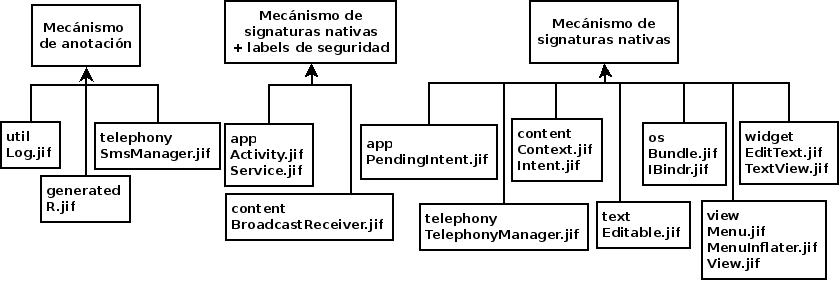
\includegraphics[width=8.5cm]{annotationsMechanims.jpeg}
	\end{center}
	\caption{Mecanismos de anotación para clases de la API.}
	\label{fig:annotationsMechanims}  
\end{figure}
dado que la API de Android provee las librerías necesarias para implementar las
funcionalidades de una aplicación Android, permitiendo a su vez, que el
aplicativo escriba o lea información de los métodos sources y sinks, las clases
pertenecientes a la API generan flujos de información. Así, para verificar la
política de seguridad previamente definida, se requieren anotaciones tanto a las
clases que definen los sources y sinks en que se centra la política, como
anotaciones a clases y librerías requeridas en la implementación de las
aplicaciones, por ejemplo, las clases que permiten implementar componentes
de actividades, servicios y broadcast receivers.\newline 
En el caso de los sinks la anotación tiene un propósito adicional, este es,
controlar el flujo de información que se envía a través de los mismos, la
definición de los métodos de las clases Log y SmsManager de la API Android,
deben anotarse de tal manera que, se controle el nivel de seguridad de los
argumentos con que se invocan tales métodos.\newline 
Para esto se utilizan las etiquetas de seguridad que regulan el llamado a
métodos en el sistema de anotaciones de Jif(sintaxis de anotación
\ref{sssec:sintaxis}), estas son Begin Label(BL) y Argument Label(AL).
Con las etiquetas para el BL se determinan los puntos del programa desde donde
puede invocarse el método, de este modo, el método podrá ser invocado si: el
nivel de seguridad del punto del programa desde donde se llama el método es
menor o igual de restrictivo que el BL con que ha sido definido el método. Para
el presente caso se busca que un método pueda ser invocado desde cualquier punto
del programa.\newline
Con las etiquetas para los argumentos del método, AL, se controla el nivel de
seguridad de los argumentos con que se invoca el método. Por tanto, el nivel de
seguridad de los argumentos con que se invoca un método, debe ser menor o igual
de restrictivo que el nivel de seguridad con que han sido definidos los
argumentos del método.\newline
El nivel de restricción de la información se evalua de acuerdo a las
etiquetas de seguridad con que de defina e invoque el método. De este modo,
información con nivel de seguridad alto es más restrictiva que información con nivel de
seguridad bajo.
Aterrizando estos conceptos a los elementos definidos en la sección
\ref{subsec:lineamientos}, información anotada con el label \emph{\{Alice:\}} es
más restrictiva que información anotada con el label \emph{\{\}}. Puesto que, el
primer label denota que la información tiene nivel de seguridad alto, mientras
que el segundo, indica que la información tiene nivel de segurodad bajo.\newline 
Tomando como ejemplo el método sendTextMessage de la clase SmsManager, mediante
el cual se envían mensajes de texto:
\begin{lstlisting}[basicstyle=\scriptsize]
sendTextMessage(String destinationAddress, String scAddress, 
	String text, PendingIntent sentIntent, 
	PendingIntent deliveryIntent){}
\end{lstlisting}

Se tiene que el parámetro \emph{text} es el que recibe la información a enviar,
y por tanto esa información debe ser pública.\newline 
Por consiguiente, en la definición del método la etiqueta de seguridad del
argumento(AL) correspondiente a la información a enviar(sms), se anota con la
etiqueta pública \{\}.
Con tal etiqueta se garantiza que la información se envía, si y sólo si, el
nivel de seguridad del argumento con que se invoca el método es menor o igual de
restrictivo que la etiqueta pública \{\}; como no se tiene una etiqueta de
seguridad menos restrictiva que esta, se garantiza que la información sólo es
envíada si efectivamente está anotada con tal etiqueta, es decir, si se trata
de información pública.\newline 
Por ejemplo,
si el método se invoca con información anotada con label de seguridad alto, se
genera un flujo de información indebido, dando lugar a un error en la
compilación del programa que le llama.\newline 
En el caso del BL al anotarlo con la etiqueta \{Alice:\}, se permite que el
método sea invocado desde cualquier punto de un programa, es decir, desde
puntos con nivel de seguridad bajo(\{\}) y desde puntos con nivel de seguridad
alto(\{Alice:\}).
Para el resto de labels se dejan los que Jif genera por defecto
\ref{sssec:default-labels}.\newline
% cualquier punto de un programa que sea igual o menor de restrictivo que el
% principal Alice, esto se traduce en que podrá ser invocado desde cualquier punto
% de un programa, lo cual es correcto porque lo que se busca el evitar que se
% envíe información considerada con nivel se deguridad alto y no, evitar que el
% método sea utilizado. Poner ejemplo XXXX?\newlie
Continuando con el ejemplo del método sendTextMessage y aplicando lo
anteriormente descrito, este método se anota de la siguiente manera:
\begin{lstlisting}[basicstyle=\scriptsize]
sendTextMessage{Alice:}(String{Alice:} destinationAddress, 
	String{Alice:}scAddress, 
	String{} text, 
	PendingIntent{Alice:} sentIntent,
	PendingIntent{Alice:} deliveryIntent) { }
\end{lstlisting}

El principio de anotación propuesto es aplicable para los métodos de la clase
Log, ya que estos también representan sinks.\newline 
Tales criterios de anotación son aplicados a través del mecanismo fundamental de
anotación que provee el sistema de anotaciones de Jif, en el cual se implementa
la respectiva versión Jif de la clase, esto es, anotando con etiquetas de
seguridad las variables, definición y cuerpo de los métodos de la clase.
Adicional a este mecanismo de anotación(mecanismo de
anotación\footnote{Para referenciar los mecanismos utilizados en la integración
de clases de la API Android, al sistema de anotaciones de Jif, se adoptan los
nombres: mecanismo de anotación, mecanismo de signaturas nativas y mecanismo de
signaturas nativas más labels de seguridad.}), el compilador de Jif provee un
mecanismo que permite interactuar con código de clases Java ya
existentes\cite{annotations-Jif}, para esto, se recurre a signaturas nativas.
Así, se implementa una versión Jif de una clase Java ya existente, en la que se
declaran signaturas nativas proveídas por Jif, constructor y métodos necesarios
de la clase(mecanismo de signaturas nativas).
Al mecanismo de signaturas nativas también se puede  adicionar labels de
seguridad(mecanismo de signaturas nativas más labels de seguridad).\newline 
% Para incluir el resto de clases de la API requeridas en la verificación de la
% política de seguridad establecida, por ejemplo, las clases que pertmiten definir
% componentes de aplicación como Activity.java(para la implementación de
% componentes de actividades), se recurre a esos mecanismos adicionales.
La figura \ref{fig:annotationsMechanims} resume las clases a anotar de acuerdo
al mecanismo con que se integran al sistema de anotaciones de Jif.
\subsubsection{Anotaciones en los aplicativos a analizar}
\label{subsec:anotador}
\begin{figure}[t!]
	\begin{center}
	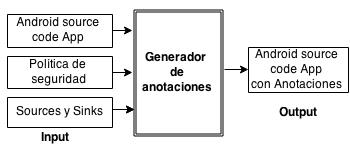
\includegraphics[width=6cm]{desingSolution2-2.jpg}
	\end{center}
	\caption{Entradas y salidas para el generador de anotaciones.\newline
	Para generar la versión anotada del aplicativo a analizar, el anotador parte
	del código fuente del aplicativo, la política de seguridad definida en
	\ref{subsection:politica} y el conjunto de sources y sinks implicados en la misma.}
	\label{fig:desingSolution}
\end{figure}
Si bien, el desarrollador debe implementar manualmente las anotaciones en el
aplicativo a análizar, acorde a las políticas de seguridad que requiere
verificar; en el presente diseño de solución, se incluye un generador de
anotaciones que automatiza la anotación requerida por el desarrollador. Como se
ilustra en la figura \ref{fig:desingSolution}, el generador de anotaciones
retorna la versión anotada del aplicativo a analizar, partiendo del código
fuente del aplicativo, la política de seguridad y el conjunto de sources y
sinks, necesarios para verificar la política de seguridad.\newline
La anotación del aplicativo se fundamenta en identificar la declaración de
sources, y en verificar qué métodos influencian esa información, de modo que,
cuando la información sea enviada a través de sinks, tenga el nivel de seguridad
adecuado. Así, las políticas de anotación definidas en \ref{subsec:elements} son
aplicadas a variables y métodos, de acuerdo a si contienen o no información del
conjunto de sources: el tipo de dato EditText\footnote{Este tipo de
dato es considerado como source si y sólo si, el campo UI al que referencia
corresponde a un campo tipo textPassword, es decir, un campo que almacena
contraseñas.} y los métodos: getDeviceId, getSimSerialNumber, findViewById,
getLatitude, getLongitude y getSubscriberId.\newline
Finalmente, se define una serie de pasos que permiten aplicar las políticas de
anotación definidas, y esos pasos son automatizados mediante el generador de
anotaciones.












